%%
%% Skript Differentialgeometrie im Wintersemester 12/13
%% Zur Vorlesung von Dr. Grensing am KIT Karlsruhe
%%
%% Uebung 12
%%

\section{4. Februar 2012}
\setcounter{Aufg}{0} %Damit die Aufgaben jedes Mal bei Aufgabe 1 anfangen
\setcounter{Loes}{0}

\begin{Aufg}
asdf
\end{Aufg}

\begin{Aufg}
asdf
\end{Aufg}

\begin{Aufg}
asdf
\end{Aufg}

\begin{Loes}\begin{description}[leftmargin=*]
\item[Operation:]
	F"ur alle $z \in E_p$ ist $S^{2k-1} \to S^{2k-1}$, $x \mapsto z.x$ stetig und f"ur alle $z, \tilde z \in E_p$ und alle $x \in S^{2k-1}$ gilt $z.(\tilde z.x) = (z \cdot \tilde z).x$.
\item[Die Operation ist frei:]
	Es ist zu zeigen dass f"ur alle $x \in S^{2k-1}$ gilt $(E_p)_x = \{1\}$, beziehungsweise f"ur alle $z \in E_p \setminus \{1\}$ und alle $x \in S^{2k-1}$ gilt $z.x \ne x$, beziehungsweise dass f"ur alle $z \in E_p$ gilt dass wenn es ein $x \in S^{2k-1}$ mit $z.x$ gibt $z=1$ gelten muss.
	Es seien $E_p$ und $(z_1,\ldots ,z_k) \in S^{2k-1}$ mit
	\begin{align*}
		(z_1,\ldots , z_k) = z.(z_1,\ldots ,z_k) = (z^{q_1} z_1, \ldots , z^{q_k} z_k)
	\end{align*}
	Da $(z_1, \ldots , z_k) \in S^{2k-1}$ ist, existiert ein $j \in \{1, \ldots ,k\}$ mit $z_j \ne 0$, und daraus folgt $z^{q_j} = 1$.
	Es seien $a,b \in \Z$ mit $1 = a q_j + b p$. Es gilt dann
	\begin{align*}
		1 = 1^a \cdot 1^b = (z^{q_j})^a (z^p)^b = z^{a q_j + b p} = z^1 = z
	\end{align*}
\item[Die Operation ist eigentlich kontinuierlich]
	Die Gruppe ist endlich und alle endlichen Gruppen operieren eigentlich diskontinuierlich, dann bleibt zu zeigen dass f"ur alle $K \in S^{2k-1}$ die Menge $\{ z \in E_p \mid z.K \cap K \ne \emptyset \}$ endlich ist.
\end{description}\end{Loes}

Der Quotient $L(p, q_1, \ldots ,q_k)$ nach dieser Operation ist also eine Mannigfaltigkeit.
F"ur $z = e^{2 \pi i \frac{l}{p}}$ ist die induzierte Abbildung eine Drehung um den Winkel $\frac{2 \pi l}{p} q_j$ in der $x_{2j-1}$-$x_{2j}$-Ebene.
Damit ist die Operation bez"uglich der Standardmetrik isometrisch und daraus folgt dass $L(p, q_1, \ldots , q_k)$ eine $\sec > 0$-Metrik besitzt.
Im Fall $p = 2$ gilt $q_1 = \ldots = q_k = 1$ und es ist $L(2, 1, \ldots ,1) = \R\P^{2k-1}$.
Laut Vorlesung gilt: F"ur $k \ge 2$ ist $S^{2k-1} \to L(p, q_1, \ldots  q_k)$ die universelle "Uberlagerung.
Dann sind die Einheitswurzeln gerade die Decktransformationsgruppe, also folgt
\begin{align*}
	\pi_1(L(p, q_1, \ldots ,q_k)) \cong E_p \cong \Z_p \cong \FakRaum{\Z}{\Z_p}
\end{align*}

\begin{kor}
Jede endlich erzeugte abelsche Gruppe ist isomorph zur Fundamentalgruppe einer kompakten Riemannschen Mannigfaltigkeit mit nichtnegativer Schnittkr"ummung.
\end{kor}

\begin{bew}
Sei $G$ eine endlich erzeugte abelsche Gruppe.
Nach dem Hauptsatz "uber endlich erzeugte abelsche Gruppen gilt:
\begin{enumerate}[label=(\arabic*)]
\item
	$G \cong \Z^l \oplus \Z_{p_1} \oplus \ldots \oplus \Z_{p_n}$
\item
	$(M, g_M)$ und $(N, g_N)$ haben die Schnittkr"ummung $\sec \ge 0$ und damit hat $(M \X N, g_M \oplus g_N)$ auch $\sec \ge 0$ (wobei $(g_M \oplus g_N)(X_M + X_N, Y_M + Y_N) = g_M(X_M + Y_M) + g_N(X_N, Y_N)$)
\end{enumerate}
Daraus folgt:
\begin{align*}
	&\pi_1(T^n \X L(p_1, 1, \ldots ,1) \X \ldots \X L(p_n, 1, \ldots , 1)) \\
	&\cong \pi_1(T^n) \oplus \pi_1(L(p_1, 1, \ldots ,1)) \oplus \ldots \oplus \pi_1(L(p_1, 1, \ldots ,1)) \\
	&\cong \Z^n \oplus \Z_{p_1} \oplus \ldots \oplus \Z_{p_n} \cong G
\end{align*}
\end{bew}

Die Mannigfaltigkeiten $L(p, q_1, \ldots ,q_k)$ und $L(p, q_1', \ldots ,q_k')$ sind:\begin{itemize}
\item
	homotopie"aquivalent genau dann wenn $q_1 \cdot \ldots \cdot q_k \equiv \pm l^k q_1' \ldots q_k' (\mmod p)$ f"ur ein $l \in \Z_p$ \cite{olum}
\item
	hom"oomorph genau dann wenn es ein $l \in \Z_p$ und ein $\sigma \in S_k$ gibt sodass f"ur alle $i$ gilt $q_i \equiv \pm l q' \sigma(i) (\mmod p)$ \textcolor{red}{(Buchverweis: E. J. Brody, 1960)}
\end{itemize}
Also handelt es sich um homotopie"aquivalente, aber nicht hom"oomorphe Mannigfaltigkeiten.

\begin{Loes}
Nach dem Korollar von Bonnet-Myers ist die Fundamentalgruppe eine vollst"andige Mannigfaltigkeit mit $\ric \ge (n-1) \kappa > 0$ endlich.
$\pi_1(T^n) = \Z^n$ nicht.
\end{Loes}

\begin{Loes}
Wir k"urzen mit (*) die rechte Seite der Behauptung ab, also
\begin{align*}
	\text{Es gibt eine Isometrie } \hat\phi: M \to M \text{, sodass } \Gamma_1 = \hat\phi \Gamma_2 \hat\phi^{-1} \tag{*}
\end{align*}
\begin{description}[leftmargin=*]
\item[\quot{$\bm{\Leftarrow}$}:]
	Es sei $\hat\phi: M \to M$ eine Isometrie mit (*).
	\marginnote{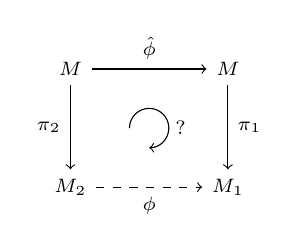
\begin{tikzpicture}[font=\scriptsize]
		\node (1) at (-1,0.75) {$M$};
		\node (2) at (1,0.75) {$M$};
		\node (3) at (-1,-0.75) {$M_2$};
		\node (4) at (1,-0.75) {$M_1$};
		\draw[->] (1) --node[above]{$\hat\phi$} (2);
		\draw[->,dashed] (3) --node[below]{$\phi$} (4);
		\draw[->] (1) --node[left]{$\pi_2$} (3);
		\draw[->] (2) --node[right]{$\pi_1$} (4);
		\draw[->] (180:0.25) arc (180:-90:0.25);
		\node at (0.4,0) {?};
	\end{tikzpicture}}
	Definiere die Abbildung
	\begin{align*}
		\phi: M_2 \to M_1 && \phi(\overset{\mathclap{\text{Bahn}}}\Gamma_2 x) = \Gamma_1 \hat\phi(x)
	\end{align*}
	\begin{description}[leftmargin=*,font=\normalfont\itshape]
	\item[Behauptung:]
		$\phi$ ist wohldefiniert
	\item[Beweis:]
		Es ist zu zeigen dass f"ur alle $\gamma_2 \in \Gamma_2$ es ein $\gamma_1 \in \Gamma_1$ gibt mit $\hat\phi(\gamma_2 x) = \gamma_1 \hat\phi(x)$.
		F"ur $\gamma_2 \in \Gamma_2$ ist $\hat\phi \circ \gamma_2 \circ \hat\phi^{-1} =: \gamma_1 \in \Gamma_1$. Dann folgt $\gamma_1(\hat\phi(x)) = \hat\phi(\gamma_2(x))$.
	\end{description}
	Die gleiche Konstruktion f"ur $\hat\phi^{-1}$ liefert $\phi^{-1}$.
	Da $\pi_i$ ein lokaler Diffeomorphismus ist folgt dass $\phi$ und $\phi^{-1}$ glatt sind.
	Da $\phi$ und $\pi_i$ lokale Isometrien sind und $\pi_2$ surjektiv ist, ist $\phi$ eine lokale Isometrie, und weil $\phi$ ein Diffeomorphismus ist folgt dass $\phi$ eine Isometrie ist.
\item[\quot{$\bm{\Rightarrow}$}:]
	Es sei $\phi: M_1 \to M_2$ eine Isometrie.
	\marginnote{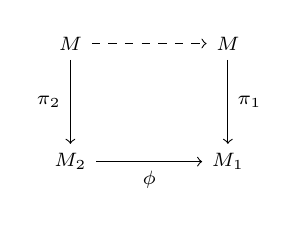
\begin{tikzpicture}[font=\scriptsize]
		\node (1) at (-1,0.75) {$M$};
		\node (2) at (1,0.75) {$M$};
		\node (3) at (-1,-0.75) {$M_2$};
		\node (4) at (1,-0.75) {$M_1$};
		\draw[->,dashed] (1) -- (2);
		\draw[->] (3) --node[below]{$\phi$} (4);
		\draw[->] (1) --node[left]{$\pi_2$} (3);
		\draw[->] (2) --node[right]{$\pi_1$} (4);
	\end{tikzpicture}}
	Dann ist $\phi \circ \pi_2$ eine lokale Isometrie, da $\phi$ ein Diffeomorphismus ist und $\pi_2$ eine "Uberlagerung, und damit ist $\phi \circ \pi_2$ eine Riemannsche "Uberlagerung.
	Aus $\pi_1(M) = \{0\}$ folgt dass $\phi \circ \pi_1$ die universelle "Uberlagerung ist; diese ist nach der Vorlesung bis auf Isomorphie eindeutig.
	Das bedeutet es existiert eine Isometrie $\hat\phi: M \to M$ mit $\pi_1 \circ \hat\phi = \phi \circ \pi_2$.
	\begin{description}[leftmargin=*,font=\normalfont\itshape]
	\item[Behauptung:] $\Gamma_1 = \hat\phi \Gamma_2 \hat\phi^{-1}$
	\item[Beweis:] \begin{description}[leftmargin=*,font=\normalfont]
		\item[\quot{$\subseteq$}:]
			\begin{align*}
				\pi_1 \circ \hat\phi \circ \gamma_2 \circ \hat\phi^{-1} = \phi \circ \pi_2 \circ \gamma_2 \circ \hat\phi^{-1} \overset{\gamma_1 \in \Gamma_2}{=} \phi \circ \pi_2 \circ \hat\phi^{-1} = \pi_1 \circ \hat\phi \circ \hat\phi^{-1} = \pi_1
			\end{align*}
		\item[\quot{$\supseteq$}:]
			\begin{align*}
				\pi_2 \circ \hat\phi^{-1} \circ \gamma_1 \circ \hat\phi = \phi^{-1} \circ \pi_1 \circ \gamma_1 \circ \hat\phi = \phi^{-1} \circ \pi_1 \circ \hat\phi = \pi_2 \circ \hat\phi^{-1} \circ \hat\phi = \pi_2
			\end{align*}
			Daraus folgt
			\begin{align*}
				\gamma_2 = \hat\phi^{-1} \circ \gamma_1 \circ \hat\phi \in \Gamma_2 && \gamma_1 = \hat\phi \circ \gamma_2 \circ \hat\phi^{-1} \in \hat\phi \Gamma_2 \hat\phi^{-1}
			\end{align*}
		\end{description}
	\end{description}
\end{description}\end{Loes}